\documentclass[10pt,a4paper]{article}
\usepackage[utf8]{inputenc}
\usepackage[a4paper,left=3cm,right=2cm]{geometry}
\usepackage{amsmath}
\usepackage[thmmarks, amsmath, thref]{ntheorem}
\usepackage{amsfonts}
\usepackage{amssymb}
\usepackage{fancyhdr}
\pagestyle{fancy}
\usepackage{anysize}
\usepackage{graphicx}
\usepackage{float}
\usepackage{hyperref}
\usepackage{pgfplots}
\pgfplotsset{compat=1.17}
\usepackage{enumitem}
\newtheorem{theorem}{Theorem}
\theoremsymbol{\ensuremath{\blacksquare}}
\newtheorem*{solution}{Solución:}

\usepackage{xcolor}

% Margenes y formalidades

\textwidth 6.25in % Margen Derecho y ancho del texto
\textheight 8.5in
\oddsidemargin 0in % Margen Izquierdo
\headheight 0in % Largo del texto
\leftmargin 1in
\parindent 0em % Salto entre la indentación (Sangría)https://www.overleaf.com/4519127669sdpptkhvsbfn
\topmargin -0.5in % Margen Superior
\parskip 0.5ex % Salto entre parrafos
\baselineskip 1pt



\lhead{
\includegraphics[scale=0.11]{Figuras/logoUSM.png}} % texto izquierda de la cabecera
%\chead{}                                      % texto centro de la cabecera
\rhead{Universidad Técnica Federico Santa María\\Ingeniería Comercial } % número de página a la derecha
\renewcommand{\headrulewidth}{0.4pt} % grosor de la línea de la cabecera
\renewcommand{\footrulewidth}{0.4pt} % grosor de la línea del pie

\begin{document}
\vspace{5cm}

\begin{center}
\begin{Large}
\textbf{\\Guía 1: Econometría ICS-294}
\end{Large}\\
\end{center}


\section{Estadística Descriptiva}

\textbf{Ejercicio 2:} Se tiene el siguiente conjunto de datos sobre el número de ventas realizadas por 5 vendedores en un mes:
$$X = \{10,15,12,18,20\}$$
Calcule la media, mediana y varianza muestral.

{\color{red} \textbf{Solución:}

La media es:
$$\Bar{X} = \frac{10+15+12+18+20}{5} = \frac{75}{5} = 15$$

Ordenando los datos: {10, 12, 15, 18, 20}, la mediana es el valor central, es decir:

$$mediana(X) = 15$$

La varianza muestral se calcula como:

$$s^2 = \frac{\sum (X_i - \Bar{X})^2}{n-1}$$

$$s^2 = \frac{(10-15)^2 + (15-15)^2 + (12 - 15)^2 + (18-15)^2 + (20-15)^2}{4}$$

$$s^2 = \frac{(-5)^2+(0)^2 + (-3)^2 +(3)^2 + (5)^2}{4} = \frac{25+0+9+9+25}{4} = \frac{68}{4} = 17$$}








\section{Muestreo}

\begin{itemize}
  \item \textbf{Muestreo aleatorio simple (MAS):} todas las unidades tienen la misma probabilidad de selección.
    \item \textbf{Sistemático:} se ordena la población y se elige un inicio aleatorio; luego cada $k$-ésima unidad. Es eficiente si no hay periodicidad alineada con $k$.
  \item \textbf{Estratificado:} la población se divide en estratos homogéneos; se muestrea aleatoriamente dentro de cada estrato y se pondera por tamaños.
  \item \textbf{Conglomerados:} se seleccionan grupos (heterogéneos internamente) y se censa o muestrea dentro de ellos; útil cuando listar individuos es costoso.
\end{itemize}

\textbf{Ejercicio 1:} Se tiene una población de 1000 individuos con una media de ingreso mensual de $1500$ y una desviación estándar de $300$. Si se toma una muestra aleatoria simple de 100 individuos, ¿cuál es la media esperada y la desviación estándar de la media muestral?

{\color{red} \textbf{Solución:}

La media esperada de la muestra es igual a la media poblacional:
$$E(\Bar{X}) = \mu = 1500$$


La desviación estándar de la media muestral (error estándar) se calcula como:

$$\sigma_{\Bar{X}} = \frac{\sigma}{\sqrt{n}} = \frac{300}{\sqrt{100}} = \frac{300}{10} = 30$$}



\section{Intervalos de confianza}

\susbsection*{Teorema del Límite Central }
Sea $X_1,\ldots,X_n$ i.i.d. con media $\mu$ y varianza finita $\sigma^2$. La media muestral $\bar X=\frac{1}{n}\sum X_i$ cumple
\[
\frac{\bar{ X}-\mu}{\sigma/\sqrt{n}} \ \xrightarrow{d}\ \mathcal{N}(0,1)\quad \text{cuando } n\to\infty.
\]
Consecuencias prácticas:
\begin{itemize}
  \item Para $n$ moderados, la distribución de $\bar{X}$ es \emph{aprox.} normal, incluso si $X_i$ no lo es.
  \item Error estándar $\operatorname{se}(\bar{X})\approx s/\sqrt{n}$, donde $s$ es la desviación estándar muestral de X.
  \item Con $\sigma$ desconocida y $n$ pequeño, usar $t$ Student.
\end{itemize}

\textbf{Ejercicio 3:} Una empresa desea comparar los tiempos promedio de producción de dos plantas, Planta A y Planta B. Se toman muestras aleatorias de los tiempos de producción (en horas) de ambas plantas.

\begin{itemize}
    \item Para la \textbf{Planta A}, se selecciona una muestra de 50 observaciones con una media muestral de \( \bar{X}_A = 5,2 \) horas y una varianza conocida de \( \sigma_A^2 = 0,16 \) horas.
    \item Para la \textbf{Planta B}, se selecciona una muestra de 60 observaciones con una media muestral de \( \bar{X}_B = 4,9 \) horas y una varianza conocida de \( \sigma_B^2 = 0,25 \) horas.
\end{itemize}

 Verifique si la diferencia entre los tiempos de producción de las dos plantas es estadísticamente significativa.

 {\color{red}
 El intervalo de confianza para la diferencia de medias con varianzas conocidas se calcula con la siguiente fórmula:

 \[
 (\bar{X}_A - \bar{X}_B) \pm Z_{\alpha/2} \cdot \sqrt{\frac{\sigma_A^2}{n_A} + \frac{\sigma_B^2}{n_B}}
\]

{\bf Paso 1: Diferencia de medias}

 \[
 \bar{X}_A - \bar{X}_B = 5.2 - 4.9 = 0.3
 \]

{\bf Paso 2: Error estándar de la diferencia de medias}

 \[
 \text{SE} = \sqrt{\frac{0.16}{50} + \frac{0.25}{60}} = \sqrt{0.0032 + 0.004167} = \sqrt{0.007367} \approx 0.0858
 \]

{\bf Paso 3: Cálculo del intervalo de confianza}

\[
 0.3 \pm 2.576 \times 0.0858
 \]

 \[
 0.3 \pm 0.2209
 \]


 El intervalo de confianza al 99\% para la diferencia de medias es:

\[
(0.0791, 0.5209)
\]


Con un 99\% de confianza, la diferencia en los tiempos promedio de producción entre las dos plantas está entre \(0.0791\) y \(0.5209\) horas. Como el valor 0 no está dentro del intervalo, se puede concluir que la diferencia es estadísticamente significativa al nivel de confianza del 99\%.
}


\section{Regresión Lineal Simple}

\textbf{Ejercicio 4:} Se tiene la siguiente muestra de datos:
\begin{center}
\begin{tabular}{|c|c|}
\hline
X (Publicidad) & Y (Ventas) \\
\hline
2 & 4 \\
\hline
4 & 7 \\
\hline
6 & 10 \\
\hline
8 & 13 \\
\hline
10 & 16 \\
\hline
\end{tabular}
\end{center}

Ajuste un modelo de regresión lineal simple de la forma:
$$Y = \beta_0 + \beta_1 X + u $$

usando el método de mínimos cuadrados ordinarios.

{\color{red} \textbf{Solución:}

Los estimadores de MCO se calculan como:
$$\hat{\beta}_1 = \frac{\sum (X_i - \Bar{X})(Y_i - \Bar{Y})}{\sum (X_i - \Bar{X})^2} = \frac{Cov(X,Y)}{Var(X)} $$
$$\hat{\beta}_0  = \Bar{Y} - \hat{\beta}_1 \Bar{X}$$

Calculamos las medias:
$$\Bar{X} = \frac{2+4+6+8+10}{5}=6$$ 
$$\Bar{Y} = \frac{4+7+10+13+16}{5} = 10$$

Calculamos $\hat{\beta}_1$ :
$$\hat{\beta}_1 = \frac{(2-6)(4-10)+(4-6)(7-10)+(6-6)(10-10)+(8-6)(13-10) + (10-6)(16-10)}{(2-6)^2+(4-6)^2+(6-6)^2+(8-6)^2+(10-6)^2}$$
$$\hat{\beta}_1 = \frac{(-4)(-6)+(-2)(-3)+(0)(0)+(2)(3)+(4)(6)}{(-4)^2+(-2)^2+(0)^2+(2)^2+(4)^2}$$
$$\hat{\beta}_1 = \frac{24+6+0+6+24}{16+4+0+4+16}= \frac{60}{40} = 1.5$$

Calculamos $\hat{\beta}_0$:
$$\hat{\beta}_0 = \Bar{Y} - \hat{\beta}_1 \Bar{X} = 10-(1.5)6 = 10 -9 = 1$$

Por lo tanto, la ecuación estimada es:

$$\hat{Y} = 1+1.5X$$}




\vspace{0.5cm}


\textbf{Ejercicio 5:} 
Se tiene un conjunto de datos que relaciona el número de horas de estudio (\(x\)) y la nota obtenida en un examen (\(y\)) por un grupo de 5 estudiantes:

\[
\begin{array}{|c|c|}
\hline
\text{Horas de estudio} (x) & \text{Nota} (y) \\
\hline
1 & 2 \\
2 & 3 \\
3 & 5 \\
4 & 4 \\
5 & 6 \\
\hline
\end{array}
\]

Se considera que la relación entre la nota obtenida y las horas de estudio 
est\'a descrita por el siguiente modelo regresión lineal poblacional:

\[
y = \beta_0 + \beta_1 x+u
\]

\begin{enumerate}
    \item  Usando el método de mínimos cuadrados, se pide calcular los estimadores de los parámetros \( \beta_0 \) y \( \beta_1 \). 

{\color{red}    Las medias de \(x\) y \(y\) son:

\[
\bar{x} = \frac{1+2+3+4+5}{5} = 3, \quad \bar{y} = \frac{2+3+5+4+6}{5} = 4
\]

{\bf Cálculo de \( \hat{\beta_1} \)}

La fórmula de \( \hat{\beta_1 }\) es:

\[
\hat{\beta_1 }= \frac{\sum (x_i - \bar{x})(y_i - \bar{y})}{\sum (x_i - \bar{x})^2}
\]

\[
\sum (x_i - \bar{x})(y_i - \bar{y}) = 9, \quad \sum (x_i - \bar{x})^2 = 10
\]

Por lo tanto:

\[
\hat{\beta_1} = \frac{9}{10} = 0.9
\]

{\bf Cálculo de \(\hat{ \beta_0} \)}

La fórmula de \( \hat{\beta_0} \) es:

\[
\hat{\beta_0} = \bar{y} - \hat{\beta_1 }\bar{x} = 1.3 =4- 0.9 \times 3 
\]}

     \item Determine los valores predichos por el modelo para las horas de estudio de la muestra y sus  residuos. Verifique que los residuos suman 0.

{\color{red}
{\bf Ecuación de la recta de regresión}

La ecuación de la recta es:

\[
\hat{y} = 1.3 + 0.9x
\]

{\bf Verificación de los residuos}

Los residuos \( \hat{u}_i = y_i - \hat{y_i} \) son:

\[
\hat{u}_1 = 2 - 2.2 = -0.2, \quad \hat{u}_2 = 3 - 3.1 = -0.1, \quad \hat{u}_3 = 5 - 4.0 = 1.0
\]
\[
\hat{u}_4 = 4 - 4.9 = -0.9, \quad \hat{u}_5 = 6 - 5.8 = 0.2
\]

Sumamos los residuos:

\[
-0.2 + (-0.1) + 1.0 + (-0.9) + 0.2 = 0
\]}
     
    \item  Compruebe que la regresión pasa por las medias de las variables x e y (es decir, el punto $(\bar{x}, \bar{y})$ está en la recta).

    {\color{red}

Debemos chequear si la recta pasa por el punto (3,4).
    \[
\hat{y} = 1.3 + 0.9\cdot 3=4  \quad 
\]}


\item Grafique la regresión lineal muestral, las observaciones de la muestra e identifique en gráfico los residuos. 

        \begin{figure}[H]
\centering
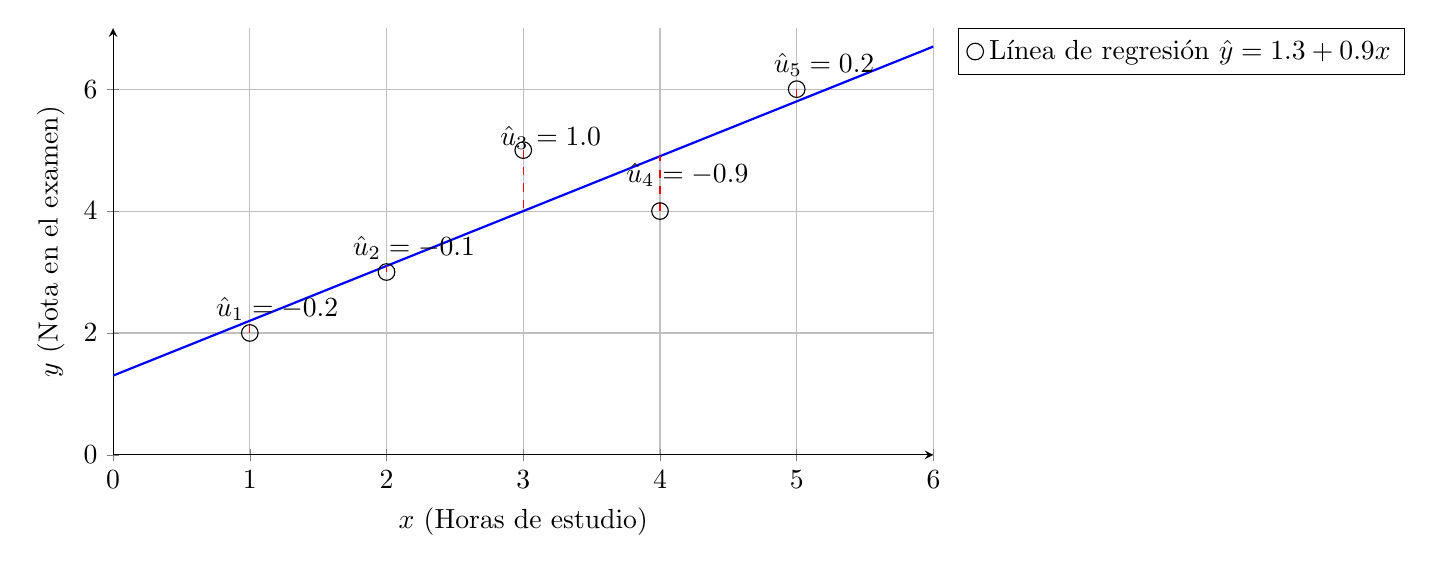
\begin{tikzpicture}
    \begin{axis}[
        axis lines = left,
        xlabel = \(x\) (Horas de estudio),
        ylabel = {\(y\) (Nota en el examen)},
        ymin=0, ymax=7,
        xmin=0, xmax=6,
        grid=major,
        width=12cm, height=7cm,
        legend pos=outer north east
    ]
    % Gráfico de los puntos
    \addplot[only marks, mark=o, mark size=3pt, black] coordinates {
        (1,2)
        (2,3)
        (3,5)
        (4,4)
        (5,6)
    };
    
    % Línea de regresión
    \addplot[domain=0:6, thick, blue] {1.3 + 0.9*x};
    \addlegendentry{Línea de regresión \( \hat{y} = 1.3 + 0.9x \)}
    
    % Líneas de los residuos (verticales)
    \draw[dashed, red] (axis cs:1,2) -- (axis cs:1,2.2);
    \draw[dashed, red] (axis cs:2,3) -- (axis cs:2,3.1);
    \draw[dashed, red] (axis cs:3,5) -- (axis cs:3,4.0);
    \draw[dashed, red] (axis cs:4,4) -- (axis cs:4,4.9);
    \draw[dashed, red] (axis cs:5,6) -- (axis cs:5,5.8);
    
    % Etiquetas de los residuos
    \node at (axis cs:1.2,2.4) {\( \hat{u}_1 = -0.2 \)};
    \node at (axis cs:2.2,3.4) {\( \hat{u}_2 = -0.1 \)};
    \node at (axis cs:3.2,5.2) {\( \hat{u}_3 = 1.0 \)};
    \node at (axis cs:4.2,4.6) {\( \hat{u}_4 = -0.9 \)};
    \node at (axis cs:5.2,6.4) {\( \hat{u}_5 = 0.2 \)};
    
    \end{axis}
\end{tikzpicture}
\caption{Regresión Lineal Muestral }
\end{figure}


\item  Determine el $R^2$ de la regresión e interprete su resultado. 

    {\color{red} La fórmula para SST es:

$SST = \sum (y_i - \bar{y})^2$

$SST = (2 - 4)^2 + (3 - 4)^2 + (5 - 4)^2 + (4 - 4)^2 + (6 - 4)^2$

$SST = (-2)^2 + (-1)^2 + (1)^2 + (0)^2 + (2)^2 = 4 + 1 + 1 + 0 + 4 = 10 $

 Ahora, calculamos SSR (Suma de Cuadrados Residual)

La fórmula para SSR es:

$SSR = \sum (y_i - \hat{y}_i)^2$

$SSR = 0.04 + 0.01 + 1.0 + 0.81 + 0.04 = 1.9$

 Calcular  finalmente, usamos la fórmula:

$R^2 = 1 - \frac{SSR}{SST}$

Sustituyendo los valores:

$R^2 = 1 - \frac{1.9}{10} = 1 - 0.19 = 0.81$



El $R^2$ es 0.81, lo que indica que el 81\% de la variación en la nota está explicada por las horas de estudio.

}
\end{enumerate}

{\bf Ejercicio 6:} Sean \(\hat{\beta}_0\) y \(\hat{\beta}_1\) el intercepto y la pendiente en la regresión de \(y_i\) sobre \(x_i\), usando \(n\) observaciones.

Ahora, sean \(\tilde{\beta}_0\) y \(\tilde{\beta}_1\) la intersección con el eje \(y\) y la pendiente en la regresión de \((c_1 + y_i)\) sobre \((c_2 + x_i)\) (sin ninguna restricción sobre \(c_1\) o \(c_2\)). Muestre que \(\tilde{\beta}_1 = \hat{\beta}_1\) y \(\tilde{\beta}_0 = \hat{\beta}_0 +c_1- c_2 \cdot \hat{\beta}_1\). Compare los $R^2$ de ambas regresiones.

{\color{red} Estimadores MCO.

$$\hat{\beta}_0 = \bar{y} - \hat{\beta}_1 \bar{x} $$
$$\hat{\beta}_1 = \frac{\sum_{i=1}^{n}(x_i - \bar{x})(y_i-\bar{y})}{\sum_{i=1}^{n}(x_i - \bar{x})^2}$$


$$\tilde{\beta}_1 = \frac{\sum_{i=1}^{n}((x_i+c_2) - (\bar{x}+c_2))((y_i+c_1)-(\bar{y}+c_1))}{\sum_{i=1}^{n}((x_i+c_2) - (\bar{x}+c_2))^2}=\hat{\beta}_1$$

$$\tilde{\beta}_0 = (\bar{y}+c_1) - \tilde{\beta}_1 (\bar{x}+c_2)= (\bar{y}+c_1) - \hat{\beta}_1 (\bar{x}+c_2)=\hat{\beta}_0+c_1-c_2\hat{\beta}_1  $$
}



    
{\color{red} SST la suma de cuadrados totales (total sum of squares):
		\[ SST = \sum_{i=1}^{n} (y_i - \bar{y})^2 \]
		
	 SSE la suma de cuadrados explicados (explained sum of squares):
	{\color{red}	\[ SSE = \sum_{i=1}^{n} (\hat{y}_i - \bar{y})^2 \]}	

 Para el segundo caso
		\[ SST' = \sum_{i=1}^{n} ((y_i+c_1) - (\bar{y}+c_1))^2 =SST\]
		
		
$$\tilde{y}_i=\tilde{\beta_0}+\tilde{\beta_1}(x_i+c_2)=\hat{\beta}_0+c_1-c_2\hat{\beta}_1 + \hat{\beta_1}(x_i+c_2)= \hat{\beta_0}+c_1+\hat{\beta_1}x_i$$
	{\color{red}	\[ SSE' = \sum_{i=1}^{n} (\tilde{y}_i - (\bar{y}+c_1))^2=SSE \]
 
 Luego el $R^2$ de ambos modelos es igual. 
 }		
  
 }


    
\section{Formulario}
\begin{itemize}

\item El intervalo de confianza de $100(1-\alpha)\%$ para la media poblacional $\mu$ cuando $\sigma$ es \emph{\textbf{conocido}}:

$$\color{red}{\bar{x} \pm z_{\frac{\alpha}{2}}\frac{\sigma}{\sqrt{n}}}$$

\item El intervalo de confianza de $100(1-\alpha)\%$ para la diferencia de medias
$\mu_x-\mu_y$ es:

$${\color{red}(\bar{X}-\bar{Y}) \pm z_{\frac{\alpha}{2}}\sqrt{\frac{\sigma_x^2}{n_x}+\frac{\sigma_y^2}{n_y}}}$$


\item El intervalo de confianza de $100(1-\alpha)\%$ para la media poblacional $\mu$ cuando $\sigma$ es \emph{\textbf{desconocido}}:

$$\color{red}{\bar{x} \pm t_{(n-1)\frac{\alpha}{2}}\frac{S}{\sqrt{n}}}$$

\item  Estimadores MCO.
{\color{red}
$$\hat{\beta}_0 = \bar{y} - \hat{\beta}_1 \bar{x} $$
$$\hat{\beta}_1 = \frac{\sum_{i=1}^{n}(x_i - \bar{x})(y_i-\bar{y})}{\sum_{i=1}^{n}(x_i - \bar{x})^2}$$}

    
\item SST la suma de cuadrados totales (total sum of squares):
	{\color{red}	\[ SST = \sum_{i=1}^{n} (y_i - \bar{y})^2 \]}
		
		\item  SSE la suma de cuadrados explicados (explained sum of squares):
	{\color{red}	\[ SSE = \sum_{i=1}^{n} (\hat{y}_i - \bar{y})^2 \]}
		
		\item  SSR la suma de cuadrados no explicados (residual sum of squares):
	{\color{red}	\[ SSR = \sum_{i=1}^{n} \hat{u}_i^2 \]}

\end{itemize}

\begin{figure}
    \centering
    
\includegraphics[width=0.9\linewidth]{figuras/normal_critic.png}

    
\end{figure}

   






\end{document}